\documentclass[margin=10pt]{standalone}
\usepackage{color,xcolor}
\usepackage{makecell}
\usepackage{tikz-qtree, tikz}
\usepackage[utf8]{inputenc}

\definecolor{myblue}{HTML}{0072BD}
\definecolor{mygreen}{HTML}{258F1B}
\definecolor{mygreendark}{HTML}{417D4D}
\definecolor{myred}{HTML}{C4000C}
\definecolor{colorNi}{HTML}{B46F84}
\definecolor{colorTi}{HTML}{3D5B7A}

\usetikzlibrary{decorations.pathreplacing,arrows,shapes,positioning,shadows,calc}
\usetikzlibrary{decorations, decorations.text,backgrounds}
\tikzset{every picture/.style={font issue=\footnotesize},
    font issue/.style={execute at begin picture={#1\selectfont}}
}

\begin{document}
\begin{tikzpicture}
% [every node/.style={inner sep=0,outer sep=60}]
    % Phases images
    \node[anchor=south west,scale=0.5,outer sep=60] (twM) at (0,0) {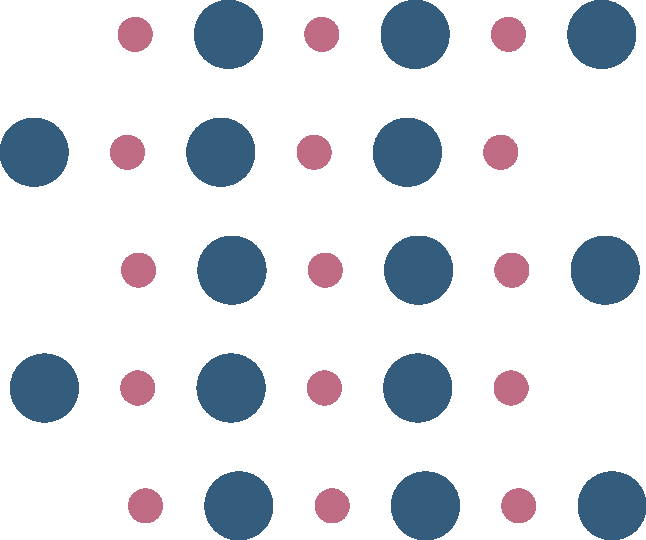
\includegraphics{twinned-martensite-phase.pdf}};
    \node[anchor=south west,scale=0.5,outer sep=60] (detwM) at (7.5,10) {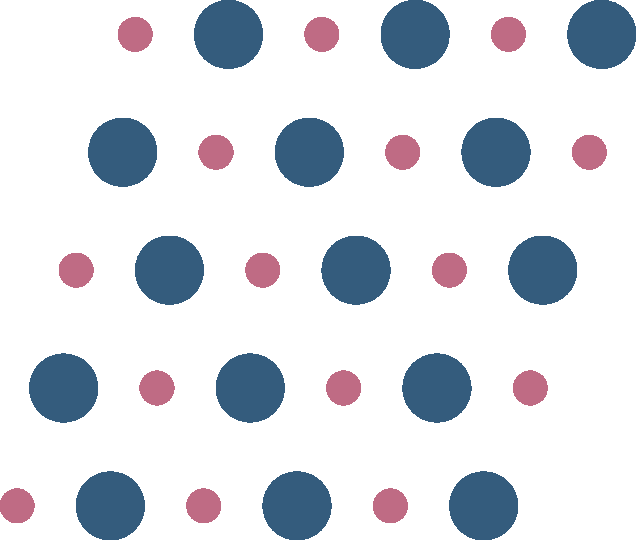
\includegraphics{detwinned-martensite-phase.pdf}};
    \node[anchor=south west,scale=0.5,outer sep=60] (A) at (15,0) {
\includegraphics{austenite-phase.pdf}};
    % Legend
    \filldraw[color=colorNi] (9.7,7) circle (4pt) node[anchor=west,outer sep=10,color=black] {\Huge Ni};
    \filldraw[color=colorTi] (11.7,7) circle (8pt) node[anchor=west,outer sep=10,color=black] {\Huge Ti};
    % Texts
    \node[anchor=center,yshift=40] (Atext)[below = of A] {\Huge Austenite};
    \node[anchor=center,yshift=50] (twMtext)[below = of twM] {\Huge\makecell[c]{Twinned\\Martensite}};
    \node[anchor=center,yshift=50] (detMtext)[below = of detwM] {\Huge\makecell[c]{Detwinned\\Martensite}};
    % Arrows
    \path [-latex,ultra thick,bend left,color=mygreendark] (twM.north) edge node [xshift=-20,pos=0.4,above,outer sep=10,color=mygreendark] {\Huge$\sigma\uparrow$} (detwM.west);
    \draw [-latex,ultra thick,color=mygreen] ($(detwM.east)+(0,0.5)$) arc(-90:180:3cm) node [xshift=30,pos=0.3,above,outer sep=10,color=mygreen] {\Huge$\sigma\downarrow$};
    \path [-latex,ultra thick, bend left,color=myred] (detwM.east) edge node [xshift=25,pos=0.6,above,outer sep=10,color=myred] {\Huge$T\uparrow$} (A.north);
    \draw [-latex,ultra thick,color=myblue] (A.west) -- node [midway,above,outer sep=10,color=myblue] {\Huge$T\downarrow$} (twM.east);

    % \path [-latex,ultra thick,out=135,in=225] (twM.north) edge (detwM.west);
    % \draw [-latex,ultra thick,out=0,in=90] ($(detwM.east)+(0,0.5)$) to [out=0,in=-90] ($(detwM.east)+(2,4)$) to [out=90, in=90 ] (detwM.north);
    % \path [-latex,ultra thick,out=0,in=90,looseness=3] ($(detwM.east)+(0,0.5)$) edge (detwM.north);
\end{tikzpicture}
\end{document}
